\documentclass{article}[11pt]
\usepackage[frenchb,english]{babel}
\usepackage[T1]{fontenc}
\usepackage[utf8]{inputenc}
\usepackage{amsmath,amssymb,latexsym}
\usepackage{times}
\usepackage{float}
\usepackage[left=2cm,right=2cm,top=2cm,bottom=2cm]{geometry}
\frenchbsetup{StandardLists=true} % � inclure si on utilise \usepackage[french]{babel}
\usepackage{enumitem}
\usepackage{fancyhdr}
\usepackage{mathrsfs}
\usepackage{graphicx}
%\usepackage[Algorithme]{algorithm}
%\usepackage{algorithmic}
\usepackage{tikz}
\usepackage{tabularx}
\usetikzlibrary{shapes}
\pagestyle{fancy}
\newcommand{\tr}[1]{{\vphantom{#1}}^{\mathit t}{#1}} 
\renewcommand\headrulewidth{1pt}
\fancyhead[L]{Cours 1�re S}
\fancyhead[R]{Yoann Pietri}
\newcounter{theoremecounter}[subsection]
\usepackage{titlesec}
\setcounter{secnumdepth}{3}% enl�ve la num�rotation apr�s les sections
%\renewcommand\thechapter {\Roman{chapter}}

 \setlength{\parindent}{0pt}

\newcommand{\R}{\mathbb{R}}
\newcommand{\N}{\mathbb{N}}
\newcommand{\Q}{\mathbb{Q}}
\newcommand{\Z}{\mathbb{Z}}
\newcommand{\C}{\mathbb{C}}
\newcommand{\K}{\mathbb{K}}
\newcommand{\eqi}{\Leftrightarrow}
\titleformat{\subsubsection}
   {\normalfont\fontsize{11pt}{13pt}\selectfont\bfseries}% apparence commune au titre et au num�ro
   {\thesubsubsection}% apparence du num�ro
   {1em}% espacement num�ro/texte
   {}% apparence du titre

\tikzstyle{theobox} = [draw=black, very thick,
    rectangle, rounded corners, inner sep=10pt, inner ysep=20pt]
\tikzstyle{theotitle} =[fill=white, text=black,rounded corners,draw=black,very thick]

\fancyhead[L]{Contrôle chapitre 5 et 6}

\usepackage{tcolorbox}
\usepackage[c]{esvect}
\newcommand{\covec}[2]{\begin{pmatrix}#1 \\#2 \end{pmatrix}}


\begin{document}
\center
\Large
Contrôle de cours
\flushleft
\center
Géométrie plane et trigonométrie
\flushleft \normalsize
Durée du contrôle : 45 min\newline
Ce sujet comporte 2 pages\newline
La calculatrice est autorisée
\subsection*{Exercice 1 (R.O.C., temps conseillé : 10 min) : }
Redémontrer la condition de colinéarité de deux vecteurs
\subsection*{Exercice 2 (temps conseillé : 20 min) : }
\center
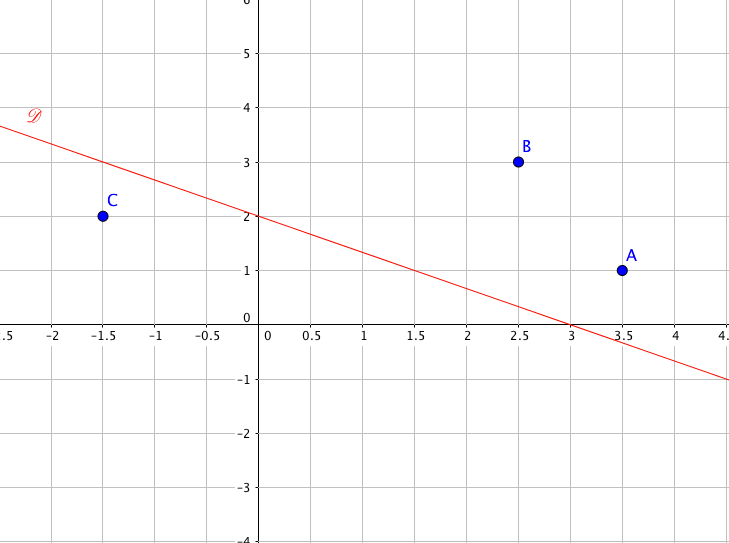
\includegraphics[scale=0.6]{chap56_ill.png}
\flushleft
\begin{enumerate}
\item Donner les coordonnées des points $A$,$B$,$C$
\item Donner les coordonnées du point $I$ milieu de $[A,B]$
\item Donner les coordonnées du vecteur $\vv{AB}$
\item Trouver un vecteur directeur de $\mathscr{D}$
\item Etablir une équation cartésienne de la droite $\mathscr{D}$
\item Trouver les coordonnées du point $D$ tel que $ABCD$ soit un parallélogramme 
\end{enumerate}
\subsection*{Exercice 3 (Coordonnées polaires, temps conseillé : 25 min) : }
\begin{enumerate}
\item Rappeler, sans démonstration, le théorème de décomposition selon 2 vecteurs non colinéaires
\item Soit $\theta \in \R$, on note $$\vv{u_\theta}= \covec{\cos(\theta)}{\sin(\theta)}$$ $$\vv{v_\theta} = \covec{-\sin(\theta)}{\cos(\theta)}$$
Montrer que $\vv{u_\theta}$ et $\vv{v_\theta}$ ne sont pas colinéaires
\item Soit $\vv{w} = \covec{x}{y}$. Déduire des questions 1 et 2 qu'il existe $\lambda$ et $\mu$ tels que $$\vv{w} = \lambda \vv{u_\theta} + \mu \vv{v_\theta}$$
\item En déduire le système 
$$\left\{\begin{array}{l l l l l} x & = & \lambda \cos(\theta) & - & \mu \sin(\theta) \quad (1) \\ y & = & \lambda \sin(\theta) & + &\mu \cos(\theta) \quad (2)\end{array}\right.$$
\item Montrer alors, en réalisant $\cos(\theta) \times (1) + \sin(\theta) \times (2)$ puis $-\sin(\theta) \times (1) + \cos(\theta) \times (2)$, on obtient 
$$\left\{\begin{array}{l} \lambda = x\cos(\theta) + y \sin(\theta) \\  \mu = y\cos(\theta) - x \sin(\theta)\end{array}\right.$$
\item Représenter $\vv{u_\theta}$ et $\vv{v_\theta}$ dans le cas $\theta = \frac{\pi}{4}$
\item Décomposer $\displaystyle \covec{\frac{1}{2}}{1}$ selon $\vv{u_\theta}$ et $\vv{v_\theta}$ dans le cas $\theta = \frac{\pi}{4}$. (\emph{On rappelle ici que $\cos(\frac{\pi}{4}) = \sin(\frac{\pi}{4}) = \frac{\sqrt{2}}{2}$})
\item A quoi correspond le cas $\theta = 0 ?$
\end{enumerate}
$$\star \star \star$$
\center
FIN DU SUJET
\end{document}